\documentclass{standalone}

\usepackage[euler-digits]{eulervm}

\usepackage{tikz}
\tikzset{every node/.style={circle,draw,minimum size=6mm,inner sep=0pt}}
\tikzset{t/.style={rectangle}}

\begin{document}
    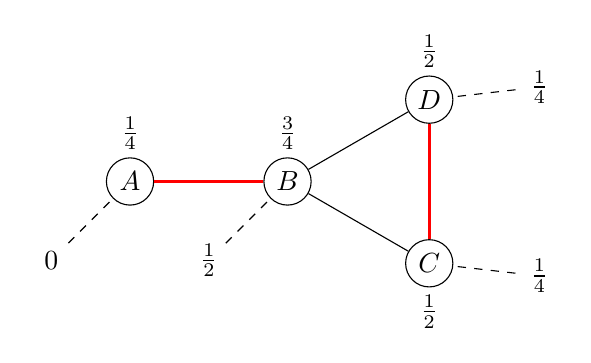
\begin{tikzpicture}[font=\sffamily]
      \node (A)[label={$\frac14$}] at (-3.2,0) {$A$}; 
      \node (B)[label={$\frac34$}] at (180:1.2) {$B$}; 
      \node (C)[label=below:{$\frac12$}] at (300:1.2) {$C$}; 
      \node (D)[label={$\frac12$}] at (60:1.2) {$D$}; 
      \node[draw=none] (a) at (-4.2,-1) {$0$};
      \node[draw=none] (b) at (-2.2,-1) {$\frac12$};
      \node[draw=none] (c) at (2,-1.2) {$\frac14$};
      \node[draw=none] (d) at (2,1.2) {$\frac14$};
      \foreach \a/\b in {B/C,D/B}
        \draw (\a) -- (\b);
      \foreach \a/\b in {A/B,C/D}
        \draw[very thick, red] (\a) -- (\b);

      \draw[dashed] (a) -- (A);
      \draw[dashed] (b) -- (B);
      \draw[dashed] (c) -- (C);
      \draw[dashed] (d) -- (D);
    \end{tikzpicture}
\end{document}
